% Internship report reconstructed from the current source code, tests, and
% mathematical proof notes in this repository. The supplied external PDF was
% used only as a visual reference for the page hierarchy and typography.
\documentclass[11pt,a4paper]{article}

\usepackage[T1]{fontenc}
\usepackage[utf8]{inputenc}
\usepackage{newpxtext}
\usepackage{amsmath,amssymb,amsthm,mathtools}
\usepackage{newpxmath}
\usepackage{microtype}
\usepackage[a4paper,top=25mm,bottom=25mm,left=27mm,right=27mm,
            headheight=15pt,headsep=8mm]{geometry}
\usepackage{graphicx}
\usepackage{booktabs,tabularx,array}
\usepackage{enumitem}
\usepackage{xcolor}
\usepackage{listings}
\usepackage{tikz}
\usetikzlibrary{arrows.meta,positioning,shapes.geometric}
\usepackage{fancyhdr}
\usepackage{hyperref}
\usepackage[nameinlink,noabbrev]{cleveref}

% -----------------------------------------------------------------------------
% Report metadata
% -----------------------------------------------------------------------------
\newcommand{\ReportTitle}{Plot Real Plane Curve Topology\\For Bivariate Polynomial}
\newcommand{\ReportShortTitle}{Plot Real Plane Curve Topology For Bivariate Polynomial}
\newcommand{\ReportSubtitle}{An Internship Report}
\newcommand{\ReportAuthor}{Dai Yuejia}
\newcommand{\ReportSupervisor}{Weijia Wang}
\newcommand{\ReportDate}{August 6, 2026}

% -----------------------------------------------------------------------------
% Typography and document style
% -----------------------------------------------------------------------------
\definecolor{ReportRed}{HTML}{981B1E}
\definecolor{ReportBlue}{HTML}{173B8F}
\definecolor{CodeGreen}{HTML}{2F6F44}
\definecolor{CodeGray}{HTML}{666666}
\definecolor{CodeBackground}{HTML}{F7F7F4}

\hypersetup{
  colorlinks=true,
  linkcolor=ReportRed,
  citecolor=ReportBlue,
  urlcolor=ReportBlue,
  pdftitle={Plot Real Plane Curve Topology For Bivariate Polynomial},
  pdfauthor={Dai Yuejia}
}

\setcounter{tocdepth}{2}
\setcounter{secnumdepth}{3}
\setlist{itemsep=0.28em,topsep=0.48em}
\setlength{\parindent}{1.25em}
\setlength{\parskip}{0pt}
\renewcommand{\arraystretch}{1.14}

\pagestyle{fancy}
\fancyhf{}
\fancyhead[L]{\small\ReportShortTitle}
\fancyhead[R]{\small\ReportAuthor}
\fancyfoot[C]{\thepage}
\renewcommand{\headrulewidth}{0.4pt}
\renewcommand{\footrulewidth}{0pt}
\fancypagestyle{plain}{%
  \fancyhf{}%
  \fancyhead[L]{\small\ReportShortTitle}%
  \fancyhead[R]{\small\ReportAuthor}%
  \fancyfoot[C]{\thepage}%
  \renewcommand{\headrulewidth}{0.4pt}%
  \renewcommand{\footrulewidth}{0pt}%
}

\newtheorem{definition}{Definition}[section]
\newtheorem{proposition}[definition]{Proposition}
\newtheorem{remark}[definition]{Remark}

\newcounter{algorithm}
\newenvironment{reportalgorithm}[1]{%
  \refstepcounter{algorithm}%
  \par\medskip\noindent
  \begin{minipage}{\textwidth}
  \hrule\vspace{0.35em}
  \textbf{Algorithm \thealgorithm}\quad #1
  \vspace{0.2em}\hrule\vspace{0.35em}
  \begin{enumerate}[leftmargin=2em,itemsep=0.16em,topsep=0.2em]
}{%
  \end{enumerate}
  \vspace{0.1em}\hrule
  \end{minipage}
  \par\medskip
}

\newcommand{\QQ}{\mathbb{Q}}
\newcommand{\RR}{\mathbb{R}}
\newcommand{\CC}{\mathbb{C}}
\newcommand{\Res}{\operatorname{Res}}
\newcommand{\Disc}{\operatorname{Disc}}
\newcommand{\lc}{\operatorname{lc}}
\newcommand{\sqfree}{\operatorname{sqfree}}
\newcommand{\Curve}{\mathcal{C}}
\newcommand{\file}[1]{\begingroup\urlstyle{tt}\path{#1}\endgroup}

\lstdefinelanguage{Julia}{
  morekeywords={abstract,break,catch,const,continue,do,else,elseif,end,export,
    false,for,function,if,import,in,let,local,macro,module,mutable,primitive,
    quote,return,struct,true,try,using,where,while},
  sensitive=true,
  morecomment=[l]{\#},
  morecomment=[n]{\#=}{=\#},
  morestring=[b]",
  morestring=[m]'
}
\lstset{
  language=Julia,
  basicstyle=\ttfamily\small,
  keywordstyle=\color{ReportBlue}\bfseries,
  commentstyle=\color{CodeGreen}\itshape,
  stringstyle=\color{ReportRed},
  numbers=left,
  numberstyle=\scriptsize\color{CodeGray},
  stepnumber=1,
  numbersep=8pt,
  frame=single,
  rulecolor=\color{black!18},
  backgroundcolor=\color{CodeBackground},
  showstringspaces=false,
  breaklines=true,
  columns=fullflexible,
  keepspaces=true,
  xleftmargin=1.5em,
  framexleftmargin=1.1em,
  aboveskip=0.8em,
  belowskip=0.8em
}

\tikzset{
  process/.style={draw=ReportBlue!65,rounded corners=2pt,fill=ReportBlue!5,
    minimum height=11mm,text width=28mm,align=center,font=\small},
  output/.style={draw=ReportRed!70,rounded corners=2pt,fill=ReportRed!5,
    minimum height=11mm,text width=28mm,align=center,font=\small},
  flow/.style={-{Latex[length=2.2mm]},thick,draw=black!65}
}

\begin{document}
\pagenumbering{gobble}

% -----------------------------------------------------------------------------
% Cover page
% -----------------------------------------------------------------------------
\begin{titlepage}
  \thispagestyle{empty}
  \centering
  \vspace*{0.20\textheight}
  {\fontsize{21}{26}\selectfont\bfseries \ReportTitle\par}
  \vspace{1.35em}
  {\Large \ReportSubtitle\par}

  \vspace{5.2em}
  {\Large \ReportAuthor\par}

  \vspace{3.0em}
  {\large Supervisor:\par}
  \vspace{0.7em}
  {\Large \ReportSupervisor\par}

  \vfill
  {\large \ReportDate\par}
\end{titlepage}

% -----------------------------------------------------------------------------
% Abstract and contents
% -----------------------------------------------------------------------------
\pagenumbering{roman}
\setcounter{page}{1}
\section*{Abstract}
\addcontentsline{toc}{section}{Abstract}

For a nonzero polynomial $P\in\QQ[x,y]$, the real zero set
$\Curve(P)=\{(x,y)\in\RR^2:P(x,y)=0\}$ may contain singularities, isolated
points, vertical components, compact loops, and unbounded branches. A numerical
contour plot can suggest its shape, but it does not certify how the branches
meet. This internship developed a Julia package that replaces a purely visual
description by a finite, exact, and testable graph representation.

The implementation first removes repeated factors and decomposes the input as
$P(x,y)=V(x)H(x,y)$, where $V$ records vertical components and $H$ is primitive
with respect to $y$. It computes projection coordinates from elimination,
isolates real algebraic points in rational boxes, and matches each box to an
exact critical abscissa. Ordinary rational fibers are then inserted between
critical fibers. The order of the real roots on a regular strip determines the
ordinary edges, while horizontal separator levels and interval refinement
certify the incidence of branches at a critical fiber. A rational coordinate
change handles projection directions in which branches may escape at a finite
abscissa. The resulting graph retains isolated vertices and can be plotted or
compactified by a single vertex at infinity. Euler's formula on the sphere then
gives the number of connected components of
$\RR^2\setminus\Curve(P)$.

The final package is organized around exact isolation, topology construction,
plotting, and region counting. Its present test suite contains fifteen passing
assertions, including circles, a line, a hyperbola, a coordinate cross, and an
isolated real point.

\paragraph{Keywords.}
Real algebraic curve; exact algebraic number; resultant; root isolation;
topology graph; certified computation; Euler characteristic; Julia.

\clearpage
\begingroup
\small
\tableofcontents
\endgroup
\thispagestyle{plain}
\clearpage

\pagenumbering{arabic}
\setcounter{page}{1}

% -----------------------------------------------------------------------------
\section{Introduction}
% -----------------------------------------------------------------------------

A bivariate polynomial is finite symbolic data, but its real zero set is a
continuous geometric object. Even low-degree examples exhibit qualitatively
different behavior: a circle is compact, a hyperbola has two unbounded
components, $xy=0$ contains a singular crossing, and $x^2+y^2=0$ consists of a
single isolated real point. A topology algorithm must distinguish these cases
without relying on the visual resolution of a plot.

The central objective of the internship was to implement the following chain:
starting from $P\in\QQ[x,y]$, compute exact finite data above its special
vertical fibers; add regular sample fibers; connect all branches with explicit
certificates; draw the resulting graph; and count the connected regions in the
complement. The active implementation is the Julia package
\file{PlotCurveTopologyForBivariatePolynomial}. Its public entry points expose
each stage separately, so intermediate results can be inspected instead of
being hidden inside one monolithic plotting command.

The work followed two development stages. The preserved rational prototype
makes the geometry visible through a hand-written Sylvester matrix, rational
root intervals, sample points, and an adjacency matrix. The active method uses
Nemo algebraic numbers, block elimination from AlgebraicSolving, Arb ball
arithmetic, separating linear projections, and rational isolating boxes. This
transition was not simply a change of numerical precision: it replaced
heuristic coordinate matching by exact equality and certified separation.

\paragraph{Main outcomes.}
The repository provides:
\begin{itemize}
  \item exact isolation of all finite topology data on special vertical
        fibers, including intersections with vertical components;
  \item explicit matching between rational boxes and exact critical
        abscissas;
  \item a topology graph that retains both edges and degree-zero vertices;
  \item certified left and right branch incidence at every critical fiber;
  \item plotting in a safe coordinate direction and mapping back to the
        original coordinates;
  \item compactification at infinity and region counting by Euler's formula.
\end{itemize}

\paragraph{Evidence boundary.}
This report is reconstructed from the current source tree, the preserved
prototype, the four proof notes, the examples, and the executable tests. No
benchmark section is included because the repository does not contain a
controlled performance study. Consequently, the validation claims concern
functional behavior and exact invariants rather than speedups.


% -----------------------------------------------------------------------------
\section{Mathematical Foundations}
% -----------------------------------------------------------------------------

\subsection{Input model and squarefree reduction}

The package accepts a nonzero polynomial $P\in\QQ[x,y]$. Repeated factors do
not change the geometric set $\Curve(P)$, so the active code first replaces
$P$ by its squarefree part
\[
  P_{\mathrm{sf}}
  =\frac{P}{\gcd(P,P_x,P_y)}.
\]
The implementation computes the greatest common divisor successively with
the derivative in each variable. This step is important because the
discriminant of a polynomial with repeated factors would otherwise vanish for
reasons unrelated to the geometry of distinct branches.

The squarefree polynomial is then decomposed as
\begin{equation}
  P_{\mathrm{sf}}(x,y)=V(x)H(x,y),
  \label{eq:vertical-decomposition}
\end{equation}
where $V$ is the monic content of $P_{\mathrm{sf}}$ with respect to $y$, and
$H$ is primitive in $\QQ[x][y]$. Every real root $\alpha$ of $V$ defines a
vertical component $x=\alpha$. The primitive part $H$ contains the remaining
curve and cannot vanish identically on an ordinary rational vertical fiber.

\subsection{Resultants and projection coordinates}

Let $F,G\in K[t]$ have degrees $m$ and $n$. Their Sylvester matrix is the
$(m+n)\times(m+n)$ matrix formed from shifted coefficient vectors of $F$ and
$G$, and the resultant is
\[
  \Res_t(F,G)=\det\bigl(\operatorname{Syl}(F,G)\bigr).
\]

\begin{proposition}[Resultant criterion]
For $F,G\in K[t]$, where $K$ is a field,
\[
  \Res_t(F,G)=0
  \quad\Longleftrightarrow\quad
  \gcd(F,G)\notin K[t]^{\times}.
\]
\end{proposition}

\begin{proof}
The Sylvester matrix represents the linear map
$(A,B)\mapsto AF+BG$ under the degree bounds
$\deg A<n$ and $\deg B<m$. Its determinant is zero exactly when a nonzero
pair $(A,B)$ lies in the kernel. If $F$ and $G$ have a nonconstant common
factor, the complementary quotients produce such a pair. Conversely, if
$AF+BG=0$ under the degree bounds and $F$ and $G$ were coprime, Euclid's lemma
would imply $F\mid B$, contradicting $\deg B<m$ unless $B=0$, and then also
$A=0$. This is the criterion developed in the corresponding proof note.
\end{proof}

For the primitive part $H(x,y)$, a vertical critical point satisfies
$H=H_y=0$. Eliminating $y$ therefore produces a univariate polynomial whose
real roots contain the corresponding critical abscissas. The package also
includes the roots of $\lc_y(H)$ because a drop of degree in $y$ may indicate
a branch that tends to infinity above a finite $x$-coordinate. The projection
set used by the proof notes is
\[
  \operatorname{proj}(H)=
  \left\{\alpha\in\RR:
    \Disc_y(H)(\alpha)=0
    \ \text{or}\ 
    \lc_y(H)(\alpha)=0
  \right\}.
\]

\subsection{Algebraic numbers and isolating boxes}

\begin{definition}
An algebraic number is a complex root of a nonzero polynomial in $\QQ[t]$.
A real algebraic number can be represented exactly together with a rational
interval that contains it and excludes every other root of its defining
polynomial.
\end{definition}

The proof notes show that algebraic numbers are closed under addition,
multiplication, additive inverses, and multiplicative inverses. This closure is essential for exact coordinate
transformations and substitutions. In the active code, Nemo's algebraic
closure of $\QQ$ represents the exact values. A bisection loop produces a
rational interval of width at most $2^{-p}$ for a requested precision $p$.

For a point $(\alpha,\beta)\in\RR^2$, the finite representation returned to
the rest of the package is an isolating box
\[
  I_x\times I_y
  = (x_{\ell},x_r)\times(y_{\ell},y_r),
\]
with rational endpoints. The code additionally retains exact algebraic
coordinates internally when equality or ordering must be certified.

\subsection{Root continuity inside a regular strip}

Let
$\alpha_1<\cdots<\alpha_s$ be the real projection coordinates of a squarefree
polynomial $H$ with positive $y$-degree. The vertical strips between consecutive
coordinates, including the two outer strips, contain no zero of
$\Disc_y(H)\lc_y(H)$.

\begin{proposition}[Constancy of real roots]
On every open regular strip $(\alpha_i,\alpha_{i+1})$, the number of distinct
real roots of $H(x,Y)$ is constant. These roots extend to continuous branches
that preserve their vertical order.
\end{proposition}

\begin{proof}
The leading coefficient does not vanish inside the strip, so every fiber is a
nonzero polynomial of fixed degree in $Y$. The discriminant does not vanish,
so every real root is simple. The implicit function theorem therefore gives a
unique local $C^1$ branch through each real point. A branch cannot stop at an
interior abscissa: its values remain locally bounded because the leading
coefficient stays away from zero, and a limiting root can again be continued
by the implicit function theorem. Local uniqueness pastes the continuations
into a branch across the strip. Distinct branches cannot cross without
creating a multiple root. Applying the continuation argument in both
directions shows that the root count is the same on any two fibers. This is
the argument developed in the regular-strip proof note.
\end{proof}

The proposition justifies a simple but powerful rule: on two ordinary fibers
in the same strip, the $k$-th root from the bottom belongs to the same branch.

\subsection{Local separation at a critical fiber}

Suppose that the finite roots on $x=\alpha$ lie in disjoint boxes ordered from
bottom to top. Choose rational horizontal levels between consecutive boxes,
and one additional level below the first and above the last.

\begin{proposition}[Horizontal separation]
Each chosen level can be kept free of the curve in a sufficiently narrow slab
around $x=\alpha$. Consequently, every nearby branch remains in a unique
horizontal window containing one critical box.
\end{proposition}

\begin{proof}
For a separator height $b$, the construction ensures $H(\alpha,b)\ne0$.
The function $x\mapsto H(x,b)$ is continuous, hence it stays nonzero on some
interval $|x-\alpha|<\varepsilon_b$. Taking the minimum over the finite set of
separator heights gives one slab in which no separator intersects the curve.
This is the local argument recorded in the branch-separation proof note.
\end{proof}

The implementation strengthens this existence statement into an explicit
certificate: it computes all real roots of each horizontal slice $H(x,b)$ and
refines the isolating interval of $\alpha$ until none of those roots lies in
the interval.

\subsection{Compactified graphs and Euler's formula}

The finite sampled graph stops unbounded branches at outer sample fibers. To
count regions, the package compactifies the plane to a sphere and joins every
unbounded branch end to one additional vertex $\infty$. Let the resulting
embedded multigraph have $V$ vertices, $E$ edges, and $C$ connected
components. Euler's formula gives
\begin{equation}
  F=E-V+C+1,
  \label{eq:euler-regions}
\end{equation}
where $F$ is the number of connected regions in
$\RR^2\setminus\Curve(P)$. Parallel edges are deliberately preserved because
they may represent different curve arcs and each contributes to $E$.


% -----------------------------------------------------------------------------
\section{From Rational Prototype to Certified Implementation}
% -----------------------------------------------------------------------------

\subsection{The rational prototype}

The directory \file{prototype/rational_method/} preserves the original
development sequence as standalone scripts. Its main components are:
\begin{itemize}
  \item extraction of polynomial coefficients and construction of a Sylvester
        matrix;
  \item determinant-based resultants and squarefree reduction;
  \item real-root isolation based on a root bound, sign variations, interval
        subdivision, and a Mobius transformation;
  \item selection of critical and ordinary sample fibers;
  \item an adjacency matrix connecting ordinary and critical sample points;
  \item conversion of the matrix to a graph for visualization.
\end{itemize}

This version made the intended geometric pipeline concrete. In particular,
it established that one does not need to sample the entire plane: it is enough
to identify special vertical fibers, insert ordinary fibers between them, and
connect compatible roots.

\subsection{Why the prototype was not the final interface}

The prototype files intentionally contain duplicated helpers and diagnostic
output. They are excluded from the package module so that historical variants
cannot overwrite the active definitions. Several design changes were required
for the current implementation:
\begin{enumerate}
  \item projected coordinates need not be rational, so a rational-only data
        model cannot represent every critical fiber exactly;
  \item nearest-point matching does not by itself certify that two samples
        lie on the same branch;
  \item an edge-only graph loses isolated real points;
  \item vertical components and branches escaping to infinity require
        separate treatment;
  \item root isolation, topology construction, plotting, and region counting
        benefit from independent interfaces and tests.
\end{enumerate}

\subsection{Architecture of the active package}

The active module loads six focused source files. The organization mirrors the
mathematical pipeline rather than the chronological order of the prototype.

\begin{table}[htbp]
\centering
\caption{Active source organization.}
\label{tab:architecture}
\begin{tabularx}{\textwidth}{@{}p{0.32\textwidth}X@{}}
\toprule
Source file & Responsibility \\
\midrule
\file{src/isolation/bivariate_real_isolation.jl}
  & Squarefree reduction, vertical decomposition, elimination, exact point
    matching, and rational isolating boxes. \\
\file{src/isolation/qbar_critical_points.jl}
  & Critical abscissas from the leading coefficient and discriminant
    resultant, represented in $\overline{\QQ}$. \\
\file{src/isolation/match_critical_boxes.jl}
  & Containment-based matching between bivariate boxes and disjoint critical
    intervals. \\
\file{src/topology/connect_critical_boxes.jl}
  & Ordinary fibers, certified incidence at critical fibers, vertices, and
    edges. \\
\file{src/plotting/plot_critical_box_edges.jl}
  & Safe coordinates, inverse mapping, and display of topology graphs. \\
\file{src/topology/count_plane_regions.jl}
  & Compactification, graph components, and Euler region counts. \\
\bottomrule
\end{tabularx}
\end{table}

The package declaration constrains Julia to version 1.10 or later and records
Nemo 0.56, AlgebraicSolving 0.11, and Plots 1 as its direct dependencies. Nemo
supplies polynomial arithmetic, algebraic numbers, factorization, resultants,
and Arb balls. AlgebraicSolving supplies block elimination, while Plots is
restricted to the presentation layer.

\subsection{Public data flow}

The active implementation exposes intermediate products instead of only a
final image. A caller can request raw isolation boxes, matched critical boxes,
all sample boxes, the full topology graph, a plot, the compactified graph, or
the final region count. This separation made the three test groups possible:
isolation can fail independently of connection, and graph construction can be
checked independently of visualization.


% -----------------------------------------------------------------------------
\section{Exact Isolation of Critical Fibers}
% -----------------------------------------------------------------------------

\subsection{Overview}

The exact isolation stage converts an infinite curve into finite algebraic
data on special fibers. The implementation does not attempt to isolate every
point of $P=0$; it isolates precisely the points needed by the topology stage.

\begin{figure}[htbp]
\centering
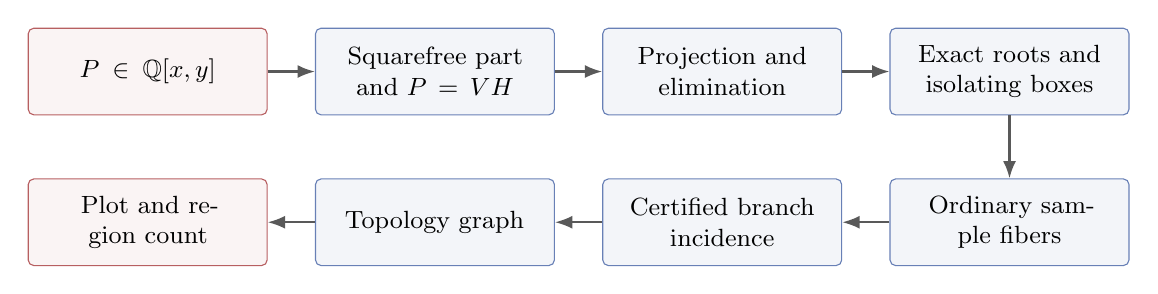
\begin{tikzpicture}[node distance=8mm and 6mm]
  \node[output] (input) {$P\in\QQ[x,y]$};
  \node[process,right=of input] (reduce) {Squarefree part and $P=VH$};
  \node[process,right=of reduce] (project) {Projection and elimination};
  \node[process,right=of project] (boxes) {Exact roots and isolating boxes};
  \node[process,below=of boxes] (samples) {Ordinary sample fibers};
  \node[process,left=of samples] (incidence) {Certified branch incidence};
  \node[process,left=of incidence] (graph) {Topology graph};
  \node[output,left=of graph] (result) {Plot and region count};
  \draw[flow] (input) -- (reduce);
  \draw[flow] (reduce) -- (project);
  \draw[flow] (project) -- (boxes);
  \draw[flow] (boxes) -- (samples);
  \draw[flow] (samples) -- (incidence);
  \draw[flow] (incidence) -- (graph);
  \draw[flow] (graph) -- (result);
\end{tikzpicture}
\caption{Data flow of the active certified implementation.}
\label{fig:pipeline}
\end{figure}

\subsection{Vertical decomposition and projection polynomial}

After computing $P_{\mathrm{sf}}$ and the decomposition in
\cref{eq:vertical-decomposition}, the main isolation routine handles two
finite systems.

First, if $\deg_y(H)>0$, it computes $H_y$ and an elimination polynomial
$C(x)$ for the ideal generated by $H$ and $H_y$. It then forms
\[
  E(x)=\sqfree\bigl(C(x)\lc_y(H)(x)\bigr).
\]
Solving $H(x,y)=E(x)=0$ returns every finite point of $H=0$ above a critical
or degree-dropping abscissa, including noncritical points on the same special
fiber. The entire fiber is retained because all of its finite roots are needed
for branch ordering.

Second, if $V$ has real roots, the system $V(x)=H(x,y)=0$ yields all
intersections between vertical components and the primitive curve. Duplicate
points belonging to both collections are removed before the boxes are
returned.

\subsection{Block elimination}

The helper \texttt{eliminationPolynomial(F,G,keep)} reorders the two variables
so that the variable to eliminate is the first block. It constructs the ideal
$\langle F,G\rangle$, calls AlgebraicSolving's block elimination, extracts
univariate candidates in the retained variable, selects the candidate of
smallest degree, and takes its squarefree part. If no univariate polynomial is
produced, the system is reported as non-zero-dimensional rather than silently
returning incomplete data.

The source also contains a direct Buchberger implementation and multivariate
normal-form helpers. They document the algebraic operations explicitly, while
the active elimination path uses AlgebraicSolving for the main computation.

\subsection{Certified coordinate matching}

Separate eliminants in $x$ and $y$ provide candidate coordinate sets, but the
Cartesian product contains false pairs. The active specialized solver reduces
this cost and certifies the correspondence as follows.

\begin{reportalgorithm}{Certified coordinate matching for $H(x,y)=q(x)=0$}
  \item Replace $q$ by its squarefree part and factor it over $\QQ$.
  \item For each irreducible factor, compute its exact real roots
        $x_1,\ldots,x_r$.
  \item Eliminate $x$ locally to obtain the possible real
        $y$-coordinates $y_1,\ldots,y_s$.
  \item Evaluate $H$ on Arb balls around each $(x_i,y_j)$. Discard a pair only
        when the resulting ball excludes zero.
  \item Search for a nonzero integer $\lambda$ such that
        $t=x+\lambda y$ separates all retained solutions.
  \item Compute the projection polynomial in $t$ and a linear relation
        $A(t)x+C(t)=0$ from a primitive pseudo-remainder sequence.
  \item Increase ball precision until every real root $\tau$ of the projection
        polynomial determines one unique candidate pair through
        $x=-C(\tau)/A(\tau)$ and $y=(\tau-x)/\lambda$.
\end{reportalgorithm}

The implementation tries $\lambda=\pm1,\ldots,\pm32$. If no projection is
certified, it retains a local exact-substitution fallback after factorization
and Arb rejection have already reduced the candidate set. Thus Arb arithmetic
is used only for certified exclusion and disjointness; final equality is never
decided by a floating-point tolerance.

\subsection{Rational isolating intervals}

For every exact real algebraic coordinate $a$, the function
\texttt{isolateAlgebraicNumber} first doubles an integer bound until
$-B\le a\le B$, then bisects rationally until the interval width is at most
$2^{-p}$. If $a$ is exactly equal to a rational midpoint, the function can
return a degenerate interval $(a,a)$. Otherwise it returns two rational
endpoints enclosing $a$.

The output of \texttt{bivariateRealIsolation(P,p)} is a sorted set of boxes
\[
  \bigl((x_{\ell},x_r),(y_{\ell},y_r)\bigr).
\]
Only finite topology data is returned. An entire vertical component cannot be
stored as a finite set of boxes, so the decomposition retains $V$ separately
for the topology stage.

\subsection{Matching boxes to exact critical abscissas}

The independent critical-coordinate path computes
\[
  \operatorname{roots}_{\RR}(\lc_y(P_{\mathrm{sf}}))
  \ \cup\ 
  \operatorname{roots}_{\RR}
  \bigl(\Res_y(P_{\mathrm{sf}},(P_{\mathrm{sf}})_y)\bigr).
\]
Each exact coordinate $\alpha$ receives a rational interval. The box-matching
routine verifies that these intervals are ordered and pairwise disjoint, then
requires every box's $x$-interval to be contained in exactly one critical
interval. Its output has the form
\[
  \bigl((\alpha,I_{\alpha}),I_y\bigr),
\]
combining an exact algebraic abscissa with rational intervals suitable for
refinement and plotting. Missing or ambiguous containment is treated as an
error, normally indicating insufficient precision.

\subsection{Isolation algorithm summary}

\begin{reportalgorithm}{Special-fiber isolation for $P\in\QQ[x,y]$}
  \item Validate that $P$ is a nonzero polynomial in exactly two variables
        over $\QQ$, and compute $P_{\mathrm{sf}}$.
  \item Compute the monic vertical content $V(x)$ and primitive part $H(x,y)$.
  \item Form the special-abscissa polynomial from elimination of
        $H,H_y$ and from $\lc_y(H)$.
  \item Solve $H=0$ above these abscissas using exact roots, Arb rejection,
        and a separating projection.
  \item Solve $V=H=0$ for intersections with vertical components.
  \item Remove duplicates, isolate every coordinate rationally, and sort the
        resulting boxes.
  \item Compute exact critical abscissas independently and match each box to
        one disjoint critical interval.
\end{reportalgorithm}


% -----------------------------------------------------------------------------
\section{Certified Topology Graph Construction}
% -----------------------------------------------------------------------------

\subsection{Graph data model}

The main interface \texttt{topologyGraphData(P)} returns
\[
  (\texttt{vertices}=\mathcal{V},\quad
   \texttt{edges}=\mathcal{E}).
\]
Every vertex is a critical or ordinary sample box. An edge is an ordered pair
of boxes representing one curve arc between consecutive sampled fibers or
along a vertical component. Keeping $\mathcal{V}$ separately is essential:
the isolated point of $x^2+y^2=0$ has degree zero and therefore cannot be
recovered from $\mathcal{E}$.

\subsection{Ordinary sample fibers}

Suppose the critical coordinates have disjoint rational isolating intervals
$I_1<\cdots<I_s$. The code selects a configurable number of rational sample
abscissas in each of the $s+1$ open strips. Bounded-strip samples are rational
fractions of the gap between consecutive critical intervals. The two outer
strips receive samples in unit-width windows just outside the first and last
critical intervals.

At an ordinary rational abscissa $\beta$, substitution produces a univariate
polynomial $H(\beta,Y)$. Its exact real roots are sorted and isolated in
$y$. This specialized path avoids running the general bivariate solver on
every sample fiber.

\subsection{Edges inside regular strips}

By the root-constancy proposition, two ordinary fibers inside the same strip
have the same number of real roots and the same vertical ordering. The code
therefore connects the $k$-th box on one fiber to the $k$-th box on the next.
If the root counts disagree, construction stops with an internal-consistency
error instead of guessing a matching. Additional samples only subdivide the
same branches and do not change their topology.

\subsection{Certified incidence at a critical fiber}

Let $B_1,\ldots,B_t$ be the boxes on $x=\alpha$, ordered from bottom to top.
The difficult step is to determine which roots immediately to the left and
right approach each $B_j$.

The code constructs disjoint horizontal windows around the boxes. A candidate
boundary is chosen rationally in every gap and is rejected if it is itself a
horizontal component of $H$. It then computes the exact roots in $x$ of every
horizontal slice $H(x,b)$. The critical interval is successively refined until
none of these roots lies over the interval. At that point no branch can cross
a window boundary in the local slab, and the ordered roots on its left and
right boundary can be assigned uniquely to windows.

\begin{reportalgorithm}{Certified incidence at $x=\alpha$}
  \item Sort the critical boxes by the midpoint of their $y$-intervals and
        verify that the intervals are disjoint.
  \item Choose one rational horizontal boundary below, between, and above the
        boxes; reject a boundary for which $H(x,b)$ is identically zero.
  \item Compute all exact real roots of each boundary polynomial $H(x,b)$.
  \item Refine the isolating interval $I_\alpha$ until no boundary root lies
        in $I_\alpha$.
  \item Evaluate the exact real roots on the left and right rational endpoints
        of $I_\alpha$.
  \item Assign each root to the unique horizontal window containing it, and
        connect it to the corresponding critical box.
\end{reportalgorithm}

A projection coordinate caused only by a vanishing leading coefficient may
have no finite box above it. In this case the adjacent branches are treated as
unbounded at the finite abscissa and receive no false finite attachment.

\subsection{Vertical components and isolated points}

For every real root $\alpha$ of $V$, the package finds the intersections of
$x=\alpha$ with $H=0$ and connects consecutive intersection boxes from bottom
to top. The two unbounded rays of a vertical component are not finite
box-to-box edges; they are accounted for later during compactification.

Isolated real points require the opposite treatment: they are retained as
vertices even though they have no incident edge. The separate vertex array is
therefore not a cosmetic interface choice but part of the topological data.

\subsection{Safe rational coordinates}

If $\lc_y(P)$ is nonconstant, a branch can escape to infinity above a finite
$x$-coordinate. Both plotting and region counting first search for a safe
rational direction. For an integer $b$, the code applies
\begin{equation}
  x=u+bv,
  \qquad
  y=-bu+v.
  \label{eq:rotation}
\end{equation}
The determinant is $1+b^2>0$, so this is an invertible linear map. If $D$ is
the total degree and $P_D$ the highest homogeneous part, the coefficient of
$v^D$ in the transformed polynomial is $P_D(b,1)$. Only finitely many integers
$b$ make this value zero. The code checks $0,-1,1,-2,2,\ldots$ until the
transformed polynomial has full $v$-degree and a nonzero constant leading
coefficient. Exact graph vertices are mapped back through
\cref{eq:rotation} before conversion to floating-point plotting coordinates.

\subsection{Complete topology algorithm}

\begin{reportalgorithm}{Construction of the sampled topology graph}
  \item Prepare $P_{\mathrm{sf}}=VH$, critical coordinates, critical boxes,
        ordinary sample abscissas, and all ordinary-fiber boxes.
  \item Connect equal-rank roots on consecutive ordinary fibers inside every
        regular strip.
  \item For each critical coordinate, certify horizontal windows and compute
        left and right branch incidence.
  \item Attach the nearest ordinary fibers to their certified critical boxes.
  \item Add edges between consecutive intersections on every vertical
        component.
  \item Sort vertices and edges while retaining degree-zero vertices and
        parallel edges.
\end{reportalgorithm}


% -----------------------------------------------------------------------------
\section{Visualization and Plane Region Counting}
% -----------------------------------------------------------------------------

\subsection{Topology plotting}

The plotting layer represents a box by its exact algebraic $x$-coordinate and
the midpoint of its rational $y$-interval, converted to \texttt{Float64} only
at the final display step. Edges are drawn as straight segments between these
representatives. They are not intended as a high-resolution approximation of
the original curve; their purpose is to make the finite topology graph visible.

The function \texttt{plotCriticalBoxes} computes the full graph, applies the
safe transformation when necessary, maps vertices and edges back to the
original coordinates, and optionally saves the result. The complete vertex
collection is passed to the scatter layer, so isolated points remain visible.

\subsection{Compactification at infinity}

The outermost ordinary fibers truncate every unbounded branch. In a safe
coordinate direction, every root on the leftmost or rightmost sampled fiber
represents exactly one unbounded end. The function
\texttt{compactifiedTopologyGraphData} creates one value of type
\texttt{PlaneInfinityVertex} and connects each such end to it. The infinity
vertex is retained even when the curve is compact; in that case it is an
isolated graph component representing the complement of the affine plane in
the sphere.

\subsection{Counting graph components and regions}

The implementation counts connected graph components with a disjoint-set
union structure using path compression and union by rank. It first validates
that every edge endpoint belongs to the vertex collection. It intentionally
does not deduplicate edges, because two arcs may have identical sampled
endpoints while enclosing a region between them.

If the compactified graph has $V$ vertices, $E$ edges, and $C$ components,
\texttt{countPlaneRegions} returns the value in \cref{eq:euler-regions}. The
zero polynomial is handled separately: its zero set is the whole plane, so the
complement has zero connected regions.


% -----------------------------------------------------------------------------
\section{Implementation and Validation}
% -----------------------------------------------------------------------------

\subsection{Principal public interfaces}

The module exports the functions in \cref{tab:api}. Precision parameters are
nonnegative, and graph construction requires the box precision to exceed the
critical-interval precision so that each box fits inside its matched interval.

\begin{table}[htbp]
\centering
\caption{Principal public interfaces.}
\label{tab:api}
\begin{tabularx}{\textwidth}{@{}p{0.46\textwidth}X@{}}
\toprule
Interface & Result \\
\midrule
\texttt{bivariateRealIsolation(P,p)}
  & Rational boxes for finite special-fiber topology data. \\
\texttt{getPointsCritical(P)}
  & Exact real algebraic projection coordinates. \\
\texttt{criticalPointBoxes(P)}
  & Critical boxes matched to exact abscissas and isolating intervals. \\
\texttt{getTopologySampleBoxes(P)}
  & All critical and ordinary sample boxes used by the graph. \\
\texttt{topologyGraphData(P)}
  & Complete sampled vertices and box-to-box edges. \\
\texttt{plotCriticalBoxes(P)}
  & A Plots.jl visualization, optionally saved to a file. \\
\texttt{compactifiedTopologyGraphData(P)}
  & Finite graph augmented by a vertex at infinity. \\
\texttt{countPlaneRegions(P)}
  & Number of connected regions in $\RR^2\setminus\Curve(P)$. \\
\bottomrule
\end{tabularx}
\end{table}

\subsection{Automated tests}

The test entry point loads three focused files. Running
\texttt{Pkg.test()} on August 6, 2026 completed all fifteen assertions:

\begin{table}[htbp]
\centering
\caption{Current automated test summary.}
\label{tab:test-summary}
\begin{tabular}{@{}lrr@{}}
\toprule
Test set & Passed & Total \\
\midrule
Exact isolation & 3 & 3 \\
Topology graph & 5 & 5 \\
Complement region counts & 7 & 7 \\
\midrule
Total & 15 & 15 \\
\bottomrule
\end{tabular}
\end{table}

The isolation tests verify that a unit circle has two critical abscissas, two
special boxes, and two matched critical boxes. The graph tests verify four
vertices and four edges for the sampled circle, retain one isolated vertex and
no edges for $x^2+y^2=0$, and confirm that the plotting interface is available.
The region tests cover two nested circles, a line, a hyperbola, a coordinate
cross, an isolated point, and the zero polynomial.

\subsection{Representative exact invariants}

For the nonzero examples, \cref{tab:cases} records the graph after
compactification. The counts were produced by the current package with
\texttt{boxPrecision=24}, \texttt{intervalPrecision=12}, and one sample per
strip. The component count follows from the same vertex and edge collection
used by the Euler calculation.

\begin{table}[htbp]
\centering
\caption{Validated compactified graph invariants and complement regions.}
\label{tab:cases}
\begin{tabularx}{\textwidth}{@{}Xrrrr@{}}
\toprule
Polynomial & $V$ & $E$ & $C$ & Regions \\
\midrule
$x^2+y^2-1$ & 5 & 4 & 2 & 2 \\
$(x^2+y^2-1)(x^2+y^2-4)$ & 17 & 16 & 3 & 3 \\
$y$ & 3 & 3 & 1 & 2 \\
$xy-1$ & 7 & 8 & 1 & 3 \\
$xy$ & 6 & 8 & 1 & 4 \\
$x^2+y^2$ & 2 & 0 & 2 & 1 \\
\bottomrule
\end{tabularx}
\end{table}

The infinity vertex explains the apparently extra graph component for a
compact curve. For the circle, for example, the sampled cycle is one component
and the isolated infinity vertex is a second component; hence
$4-5+2+1=2$ regions. For the isolated point, both the finite point and infinity
are isolated vertices, so $0-2+2+1=1$.

\begin{figure}[htbp]
\centering
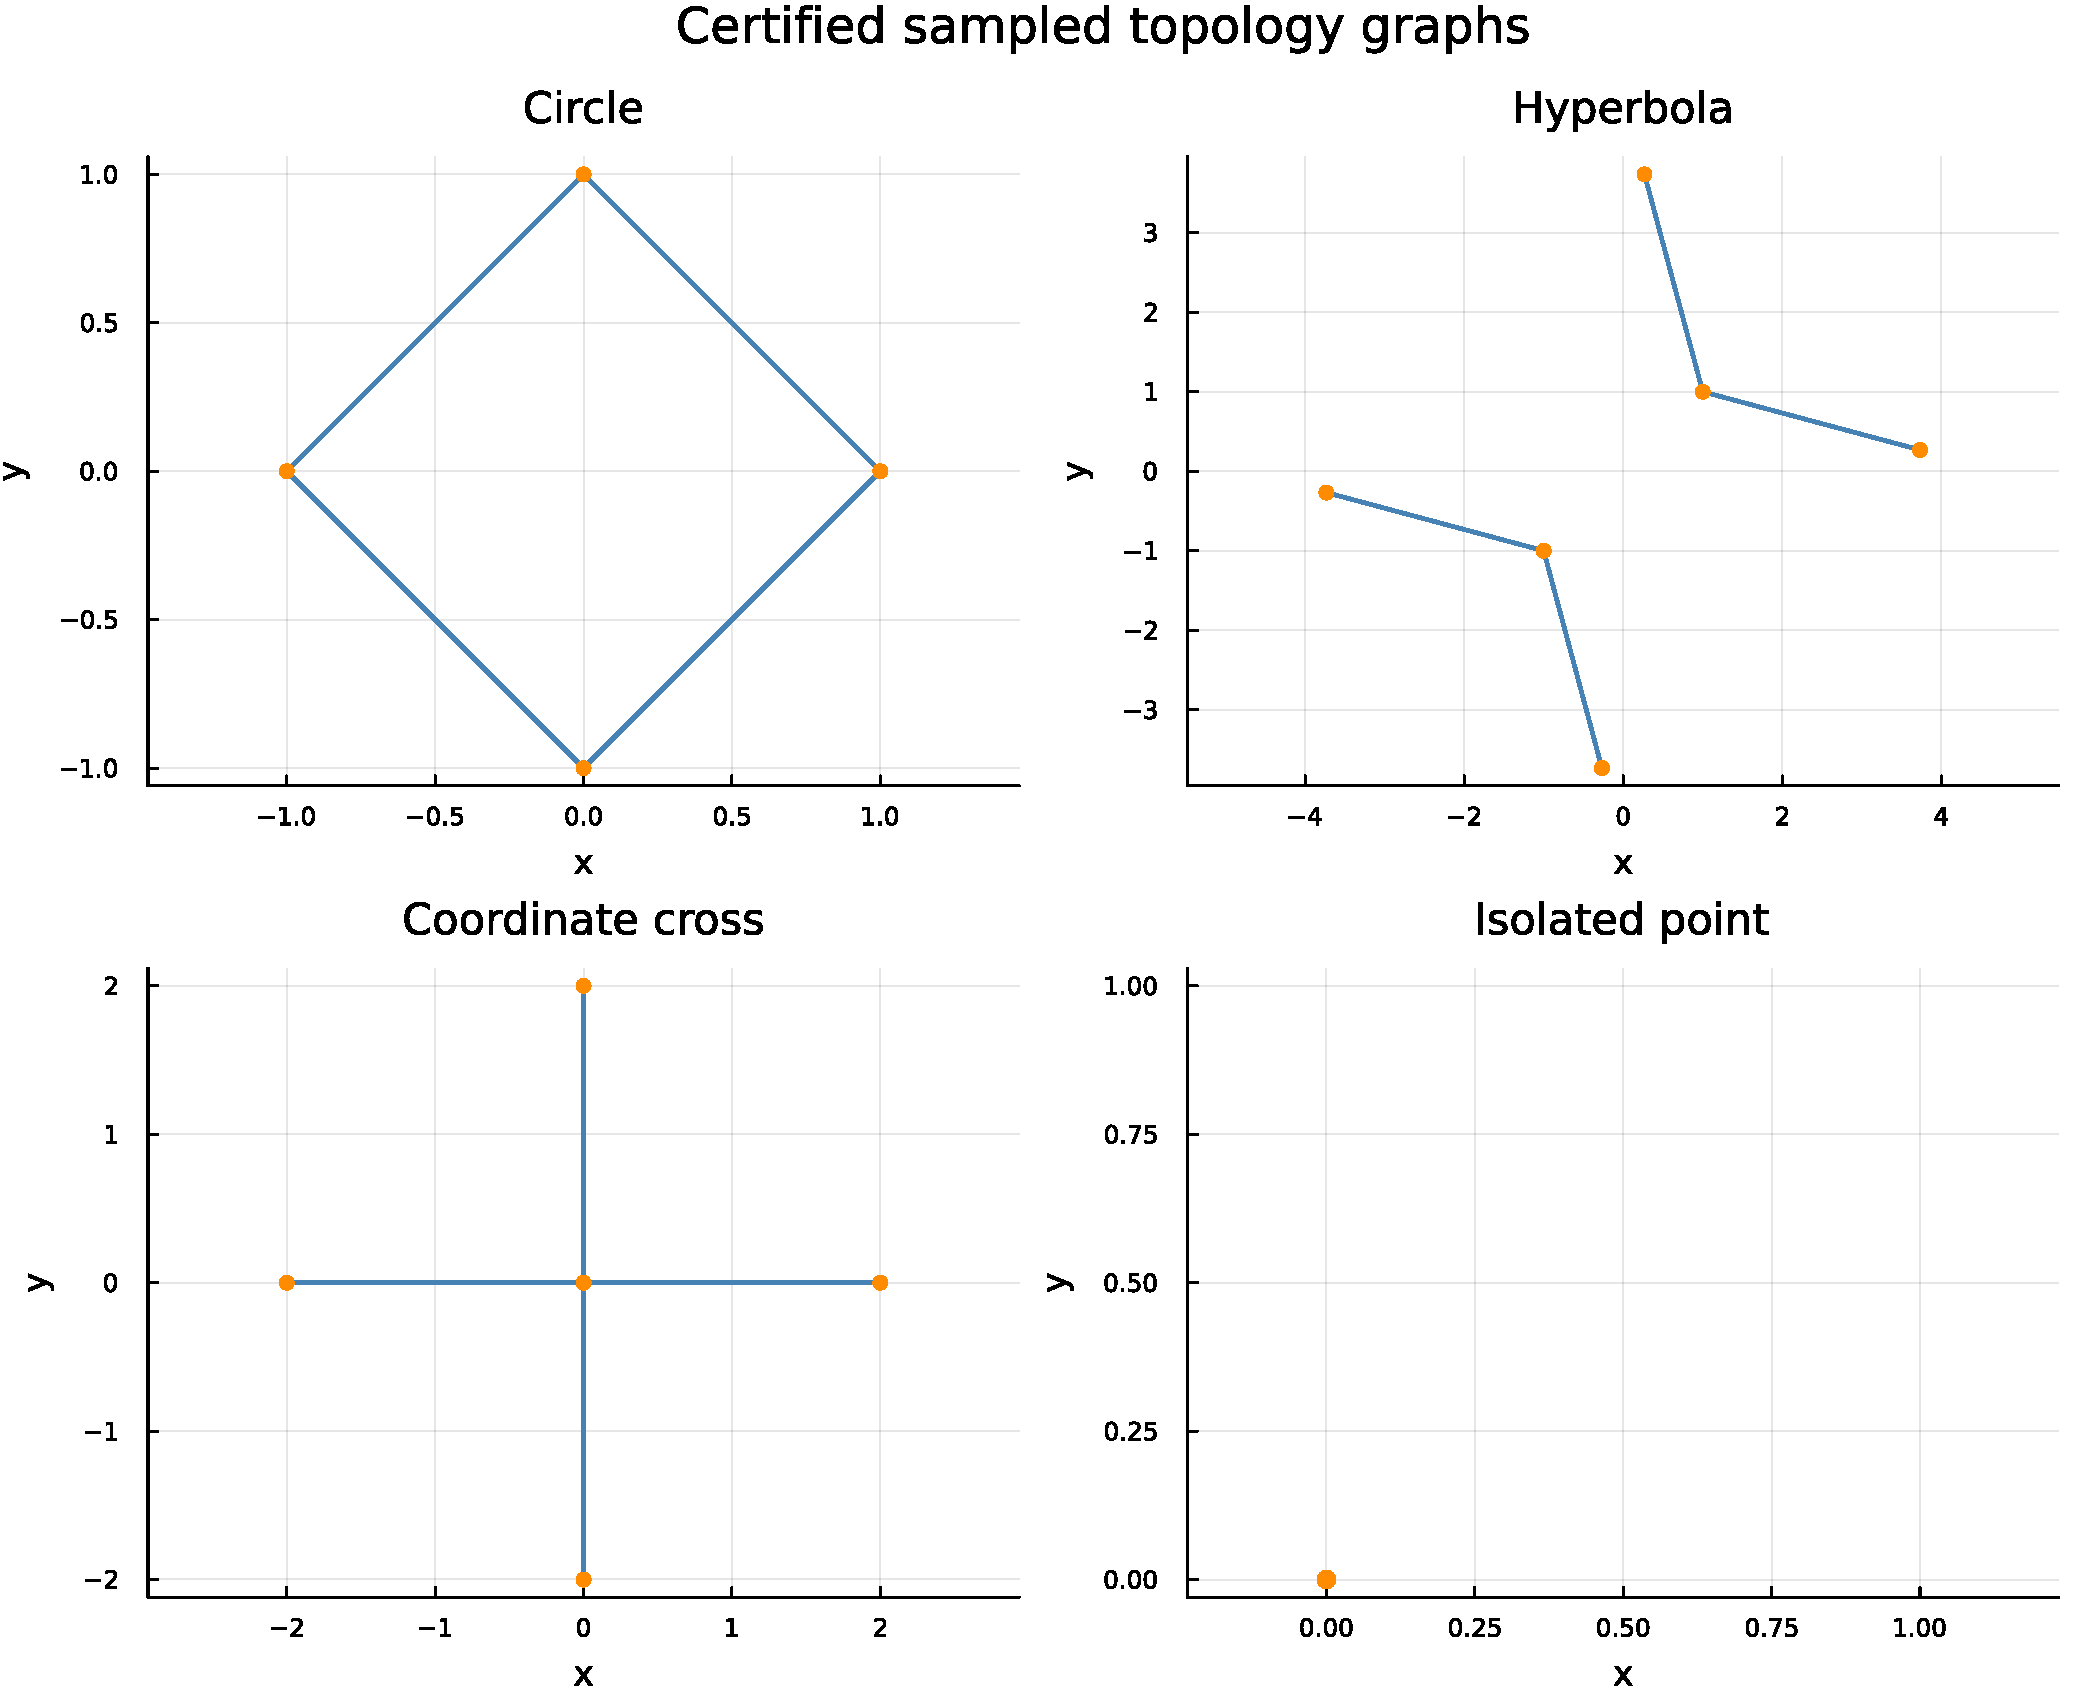
\includegraphics[width=\textwidth]{figures/validation_gallery.pdf}
\caption{Topology-graph visualizations generated by the current package. The
straight segments represent certified sampled adjacency, not a numerical
contour approximation.}
\label{fig:gallery}
\end{figure}
\clearpage

\subsection{Correctness mechanisms visible in the source}

The active code contains explicit guards at the points where a heuristic
implementation would commonly make an unchecked assumption:
\begin{itemize}
  \item input rings, variable counts, nonzero conditions, and precision
        parameters are validated;
  \item critical intervals must be ordered and pairwise disjoint;
  \item every bivariate box must match exactly one critical interval;
  \item y-intervals on a critical fiber must be disjoint;
  \item ordinary fibers in one strip must have equal root counts;
  \item horizontal separators must be certified clear of the local slab;
  \item a separating projection must produce a bijection with candidate
        coordinate pairs;
  \item all graph edge endpoints must occur in the vertex collection.
\end{itemize}

These checks do not replace a complete formal proof of the program, but they
turn the main mathematical preconditions into executable failure conditions.

\subsection{Current limitations}

The present scope is deliberately narrower than a general-purpose real
algebraic geometry library:
\begin{itemize}
  \item the public input model is restricted to $\QQ[x,y]$;
  \item exact elimination and algebraic-number comparisons may dominate the
        cost for high-degree or dense inputs;
  \item the specialized separating projection tries a finite list of small
        integer slopes before using exact substitution as a fallback;
  \item local incidence may require higher box precision or more interval
        refinements on difficult inputs;
  \item the automated suite covers representative geometries but remains
        small and contains no randomized regression corpus;
  \item the repository contains no controlled timing benchmark, so no
        performance comparison is claimed in this report.
\end{itemize}


% -----------------------------------------------------------------------------
\clearpage
\section{Conclusion}
% -----------------------------------------------------------------------------

The internship produced an end-to-end implementation for real plane
algebraic curves over $\QQ$. The final workflow begins with squarefree
reduction and vertical decomposition, obtains exact projection coordinates,
isolates finite special points in rational boxes, certifies branch incidence,
builds a topology graph, draws the graph in the original coordinates, and
counts complement regions after compactification. The development path from a
rational prototype to an exact package is preserved in the repository and
explains the major interface decisions of the active code.

The most important design principle is the separation of exact computation
from presentation. Algebraic equality, ordering, exclusion, and incidence are
resolved before any conversion to floating point. Plotting then becomes a view
of already-computed topology rather than evidence for it. The explicit vertex
collection likewise separates the mathematical graph from an edge-only
visualization and makes isolated points first-class results.

\end{document}
